\documentclass[a4paper, 11pt]{article}

\usepackage{enumitem}
\usepackage{graphicx}
\usepackage{hyperref}
\usepackage[utf8]{inputenc}
\usepackage{minted}

\begin{document}

\title{
	\textbf{Trees in C}
}
\author{Neo Gullberg}
\date{Fall 2024}
\maketitle

\section{Introduction}
	My task for this assignment was to implement functionality for working with trees in the C programming language.
	Trees build upon the concept of linked lists which we have explored in a previous assignment.
	This time we will look at binary trees specifically.

\section{Binary Tree Representation}
	Trees are made up of nodes.
	The nodes themselves hold some kind of value, in addition to pointers which branch out to further nodes.
	It is important that the value is comparable, since comparisons are important for traversing trees effectively.
	In the case of binary trees, one node contains two branches.
	If all branches for a given node are \texttt{NULL} pointers, that node is called a leaf.
	This is how I represented a node in my code:
	\begin{minted}[tabsize=4]{c}
struct Node
{
	int value;
	Node *left;
	Node *right;
};
	\end{minted}
	The structure representing a tree only contains the first (root) node:
	\begin{minted}[tabsize=4]{c}
struct Tree
{
	Node *root;
};
	\end{minted}

\section{Adding Nodes to a Tree}
	It is useful to be able to add nodes to our tree.
	And when we do, we want the tree to remain sorted.
	I ended up creating two functions for adding to a tree: one with recursion, and one without.
\subsection{Recursive Approach}
	\begin{minted}[tabsize=4]{c}
void Tree_add_recursive(Tree *tree, int value)
{
	Node_add(&tree->root, value);
}

void Node_add(Node **node, int value)
{
	if (*node == NULL)
		*node = Node_construct(value);
	else
	{
		if (value < (*node)->value)
			Node_add(&(*node)->left, value);
		else if (value > (*node)->value)
			Node_add(&(*node)->right, value);
	}
}
	\end{minted}
	For the recursive approach I used two functions,
	since one function wouldn't have been able to handle both cases of either a tree or a node without some compromise.
	First we check if the node points to \texttt{NULL}, and if so we construct a new node and let it point to that one.
	Otherwise, we compare the value we want to add, \textit{a}, with the value of the node, \textit{b}.
	If \(a < b\) then we traverse the left side,
	if \(a > b\) we traverse the right side,
	and if \(a = b\) we don't do anything since that means the value already exists in the tree.
\subsection{Non-recursive Approach}
	\begin{minted}[tabsize=4]{c}
void Tree_add(Tree *tree, int value)
{
	Node **current = &tree->root;
	while (*current != NULL)
	{
		if (value < (*current)->value)
			current = &(*current)->left;
		else if (value > (*current)->value)
			current = &(*current)->right;
		else // value already exists
			return;
	}
	*current = Node_construct(value);
}
	\end{minted}
	The logic for the non-recursive approach is basically the same.
	They both traverse the tree, following the same logic,
	until they stumble upon a \texttt{NULL} node and create a new node with the given value for that one to point to.
	The difference being that we use a while loop here, instead of relying on the implicit program stack like recursion has to.
\subsection{Benchmark}
	\begin{figure}[H]
		\centering
		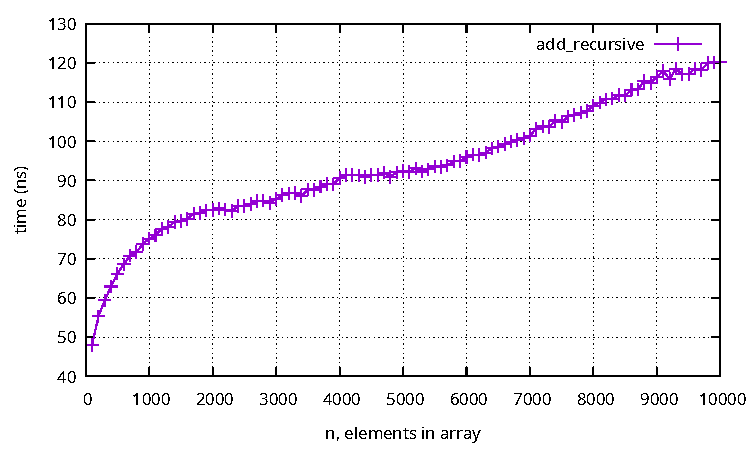
\includegraphics[scale=0.8]{graphs/add_recursive.pdf}
		\caption{
			Graph showing the time it took to add an element to a tree of size \(n\) using recursion.
			Looks to have a time complexity of \(O(\log n)\).
		}
	\end{figure}
	\begin{figure}[H]
		\centering
		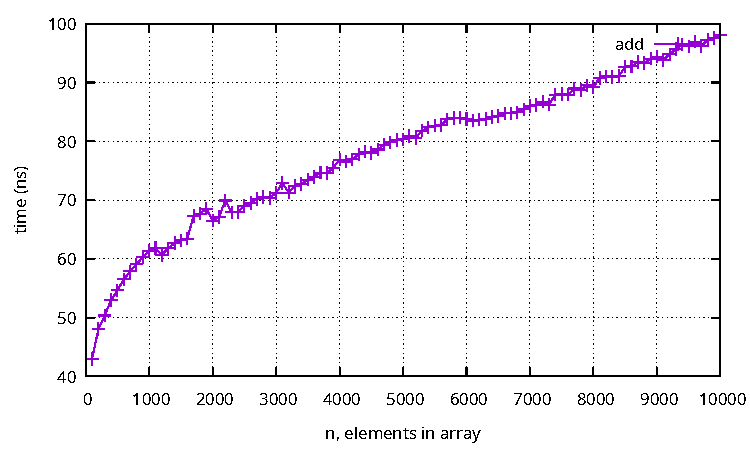
\includegraphics[scale=0.8]{graphs/add.pdf}
		\caption{
			Graph showing the time it took to add an element to a tree of size \(n\) without using recursion.
			Looks to have a time complexity of \(O(\log n)\).
		}
	\end{figure}
	It looks like the non-recursive approach seems to be a little faster,
	and in my opinion it was also a little bit easier to implement.
	The reason for it being a little faster is likely due to it not having to rely on the implicit stack.

\section{Lookup}
	The lookup method I wrote is very similar to the add method.
	It could very well have been implemented using recursion, but I chose not to.
	\begin{minted}[tabsize=4]{c}
bool Tree_lookup(Tree *tree, int value)
{
	Node **current = &tree->root;
	while (*current != NULL)
	{
		if (value < (*current)->value)
			current = &(*current)->left;
		else if (value > (*current)->value)
			current = &(*current)->right;
		else
			return true;
	}
	return false;
}
	\end{minted}
	\begin{figure}[H]
		\centering
		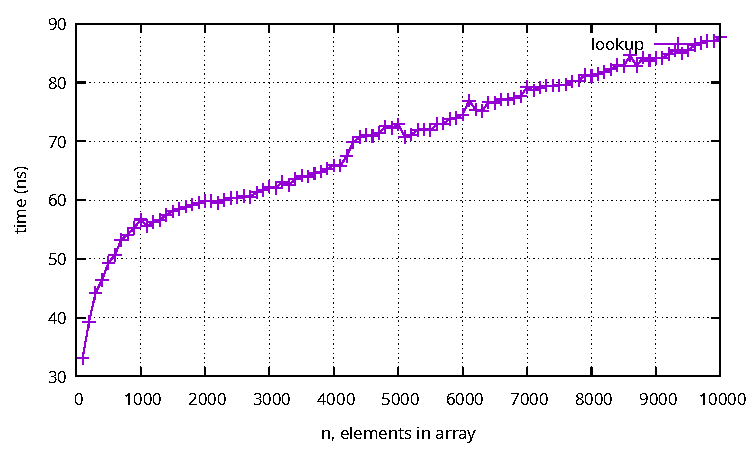
\includegraphics[scale=0.8]{graphs/lookup.pdf}
		\caption{
			Graph showing the time it took to find an element in a tree of size \(n\).
			Looks to have a time complexity of \(O(\log n)\).
		}
	\end{figure}
	Similar to that of the binary search algorithm which we benchmarked in a previous assignment,
	this also looks to have a time complexity of \(O(\log n)\).

\section{Printing Using an Explicit Stack}
	We were asked to implement a print procedure that would print out each element in the tree from left to right.
	The caveat being we were not allowed to use the implicit program stack.
	The dynamic stack that I used for this was adapted from the stack I implemented in one of the earliest assignments,
	and improved from my knowledge of linked lists.
	\begin{minted}[tabsize=4]{c}
void Tree_print_with_explicit_stack(Tree *tree)
{
	if (tree == NULL || tree->root == NULL) return;

	Stack *stack = Stack_construct();
	Node *current = tree->root;

	// moving to the leftmost node
	while (current->left != NULL)
	{
		Stack_push(stack, current);
		current = current->left;
	}

	while (current != NULL)
	{
		printf("%i\n", current->value);

		if (current->right != NULL)
		{
			current = current->right;
			while (current->left != NULL)
			{
				Stack_push(stack, current);
				current = current->left;
			}
		}
		else
		{
			pop_result result = Stack_pop(stack);
			current = result.valid ? result.value : NULL;
		}
	}

	Stack_destruct(stack);
}
	\end{minted}
	We start by traversing to the leftmost node and pushing each node one the way to the stack.
	Then we print the value at that node.
	If the right branch of the node we are at is not \texttt{NULL} we repeat the process for that branch.
	If we ever encounter a right branch that is \texttt{NULL} we start popping the stack and processing those nodes.
	This whole process repeats until all nodes have been printed.

\section{Source Code}
	If anyone is interested, the source code for this project can be found over at:
	\url{https://github.com/neogulgul/ID1021/tree/main/trees}

\end{document}
